\documentclass{article}

\usepackage[utf8]{inputenc} 
\usepackage[T1]{fontenc}
\usepackage[french]{babel}
\usepackage[margin=2.5cm]{geometry}
\usepackage{hyperref}
\usepackage{graphicx}
\usepackage[ruled,linesnumbered]{algorithm2e}
\usepackage{xcolor}
\usepackage{amsmath}
\usepackage{amssymb}

\newcommand{\pluseq}{\mathrel{+}=}
\newcommand{\minuseq}{\mathrel{-}=}
\newcommand\comm[1]{\footnotesize\ttfamily\textcolor{gray}{// #1}}

\title{Projet C++ : problème du sac à dos à choix multiple et politique d'incitations}
\author{\textsc{Javaudin} Lucas, \textsc{Le Rest} François}

\begin{document}

\maketitle

\tableofcontents

\newpage

\section{Introduction}

En recherche opérationnelle, le problème du sac à dos\footnote{Voir \url{en.wikipedia.org/wiki/Knapsack_problem}} est un problème d'optimisation dont l'objectif est de maximiser la valeur des objets que l'on insère dans un sac qui ne peut pas supporter plus d'un certain poids.

Nous étudions ici une variante du problème du sac à dos : le problème du sac à dos à choix multiple ou \textit{multiple choice knapsack problem} (MCKP).
Dans le MCKP, les objets sont regroupés en plusieurs classes et le sac à dos doit être rempli avec un et un seul objet de chaque classe.

Le MCKP est un problème NP-complet.
Nous proposons plusieurs algorithmes qui donnent une approximation de la solution optimale.
Plus précisément, les solutions proposées par ces algorithmes sont réalisables et leur distance par rapport à la solution optimale est bornée.

Enfin, nous montrons que le problème du sac à dos à choix multiple est équivalent au problème consistant à trouver la politique d'incitations maximisant l'utilité sociale, lorsque les individus font face à un choix discret et lorsque le budget de la politique est contraint.

\newpage
\section{Algorithmes}
% On peut mettre ici un pseudo-code des algorithmes que l'on a codé.

\subsection{Recherche exhaustive}

L'algorithme de recherche exhaustive parcourt toutes les allocations possibles et renvoie l'allocation optimale, c'est-à-dire l'allocation qui a la plus grande valeur parmi toutes les allocations dont le poids ne dépasse pas la capacité du sac à dos.

Cet algorithme est NP-hard.
En effet, si l'on note $J$ le nombre de classes et $n$ le nombre d'objets dans chaque classe, alors le nombre d'allocation possible est $n^J$.\footnote{Nos algorithmes autorisent un nombre d'objets différent dans chaque classe. Dans ce cas, le nombre d'allocation possible est $n_1 \cdot \dots \cdot n_J$ où $n_i$ est le nombre d'objets dans la classe $i$.}

Pour parcourir toutes les allocations, on ordonne les objets dans chaque classe et on commence par l'allocation qui prend le premier objet de chaque classe.
Pour obtenir l'allocation suivante, on prend l'objet suivant de la première classe.
Si l'on atteint le dernier objet de la première classe, alors on prend l'objet suivant de la deuxième classe (si ce n'est pas le dernier de la classe), et ainsi de suite.
La table \ref{tab:recherche-exhaustive} montre comment l'algorithme parcourt toutes les allocations lorsque qu'il y a trois classes avec trois objets dans chaque classe (les objets sont indicés 0, 1 et 2).

\begin{table}[!ht]
	\centering
	\caption{Fonctionnement de la recherche d'allocation pour $J=3$ et $n=3$}
	\label{tab:recherche-exhaustive}
	~\\
	\begin{tabular}{c|ccc}
		& Classe 1 & Classe 2 & Classe 3\\
		\hline
		Allocation 1 & 0 & 0 & 0\\
		Allocation 2 & 1 & 0 & 0\\
		Allocation 3 & 2 & 0 & 0\\
		Allocation 4 & 0 & 1 & 0\\
		Allocation 5 & 1 & 1 & 0\\
		Allocation 6 & 2 & 1 & 0\\
		Allocation 7 & 0 & 2 & 0\\
		Allocation 8 & 1 & 2 & 0\\
		Allocation 9 & 2 & 2 & 0\\
		Allocation 10 & 0 & 0 & 1\\
		$\vdots$ & $\vdots$ & $\vdots$ & $\vdots$\\
	\end{tabular}
\end{table}

L'algorithme \ref{alg:recherche-exhaustive} est un pseudo-code de l'algorithme implémenté en C++.

\begin{algorithm}[!ht]
\caption{Algorithme de recherche exhaustive pour le MCKP.}
\label{alg:recherche-exhaustive}
\small
\SetKwInOut{Input}{Input}\SetKwInOut{Output}{Output}
\Input{$J$ classes avec $n_j$ objets dans chaque classe, capacité $c$}
On note $\mathbf{x} = (x_1, \dots, x_J)$ l'allocation actuelle.\\
Dans chaque classe, on choisit l'objet d'indice 0 : $x_j = 0$, $\forall j$.\\
$\tilde{j}=0$ \comm{Classe modifiée lors de la recherche d'une nouvelle allocation.}\\
$\mathbf{x}^{*} = $ null \comm{Allocation optimale.}\\
$v^{*} = 0$ \comm{Valeur totale de l'allocation optimale.}\\
\While{$\tilde{j} < J$}
{
	\comm{On cherche l'allocation suivante.}\\
	$\tilde{j} = 0$\\
	\While{true}
	{
		\eIf{$x_{\tilde{j}} < n_{\tilde{j}}$}
		{
			On choisit l'objet suivant dans la classe $\tilde{j}$ : $x_{\tilde{j}} \pluseq 1$.\\
			\textbf{break}
		}
		{
			On reprend l'objet d'indice 0 dans la classe $\tilde{j}$ : $x_{\tilde{j}} = 0$.\\
			On s'intéresse à la classe suivante : $\tilde{j} \pluseq 1$.
		}
	}
	\comm{On regarde si la nouvelle allocation est l'allocation optimale.}\\
	$w =$ poids total de l'allocation $\mathbf{x}$\\
	\uIf{$w < c$}
	{
		$v =$ valeur totale de l'allocation $\mathbf{x}$\\
		\uIf{$v > v^{*}$}
		{
			$v^{*} = v$\\
			$\mathbf{x}^{*} = \mathbf{x}$\\
		}
	}
}
\Output{Allocation $\mathbf{x}^{*}$}
\end{algorithm}

\newpage
\subsection{Algorithme Greedy simple}
L'algorithme Greedy simple fournit une approximation de l'allocation optimale. Pour réduire le nombre de combinaison à tester, cet algorithme se base sur deux concepts : la domination et l'efficacité.\\
Soient deux objets $x$ et $y$ de la même classe. Alors on dit que que l'objet $y$ est dominé par $x$ si, par définition, on a $w_{x} \leq w_{y}$ et $p_y \leq p_x$. L'élimination des objets dominés n'a pas d'impact sur l'optimalité de l'output rendu par l'algorithme, car un objet dominé ne sera jamais présent dans l'allocation optimale.

L'efficacité d'un objet $x$ par rapport à un objet $y$ de la même classe est, quant à elle, définie par :
\begin{equation}\label{eq:eff}
    e_{x,y} = \frac{p_x - p_y}{w_x - w_y}.
\end{equation}
À chaque itération, nous allons chercher l'objet maximisant l'efficacité par rapport à l'objet de la même classe présent dans l'allocation $x^*$ :
\[ r_j = \underset{x\in C_j}{\arg\max}\ e_{x,x_j},\] où $x_j$ est l'objet de la classe $j$ dans le sac à dos.\\
En notant $\mathbf{r}=\left(r_1,\dots,r_J\right)$, on définit alors le meilleur remplaçant $r^*$ par :
\[ r^* = \underset{j=1,\dots,J}{\arg\max}\ r_j.\]
On itère jusqu'à ce que le poids maximal soit dépassé ou qu'il n'y ait plus de remplaçant (si on change d'objet optimal dans la classe $j^*$, on retire tous les objets de $j^*$ de poids inférieur à $r^*$). 

L'algorithme \ref{alg:greedy-simple} est un pseudo-code de l'algorithme implémenté en C++.

\begin{algorithm}[!ht]
\caption{Algorithme Greedy simple.}
\label{alg:greedy-simple}
\small
\SetKwInOut{Input}{Input}\SetKwInOut{Output}{Output}
\Input{$J$ classes avec $n_j$ objets dans chaque classe, capacité $c$}
	On note $\mathbf{x}^{*} = (x_1, ,., x_{J})$ l'allocation optimale.\\
	\For{classe $j$ dans $\{1, \dots, J\}$}
	{
	    On retire les objets dominés par un autre objet de la classe.\\
	    On choisit pour $x_j$ l'objet le plus léger de la classe.\\
	    On calcule $r_j = \underset{x\in C_j}{\arg\max}\ e_{x,x_j}$.
	}
	
	\While{il reste au moins un remplaçant dans une classe et $c>0$}
	{
	    On prend $r^*$ et on note $j^*$ sa classe.\\
	    On calcule la prise de poids du sac $d_w = w_y-w_{x_j}$.\\
		\eIf{$d_w \leq c$}
		{
			On retire $x_{j^*}$ de $C_{j^*}$ ainsi que\\
			On change d'objet pour la classe $j$ : $x_j = r^*$.\\
			On diminue la capacité restante $c \minuseq d_w$.\\

			\For{objet $x$ dans la classe $j^*$}
			{
				\uIf{$w_x \leq w_{r^*}$}
				{
					On retire $x$ de la classe.\\
				}
			}
			On calcule le nouveau $r_{j^*} = \underset{x\in C_{j^*}}{\arg\max}\ e_{x,r^*}$. \\
		}
	    {
	    On fixe $c=0$ pour arrêter l'algorithme.
	    }
	}
\Output{Allocation $\mathbf{x}^{*}$}
\end{algorithm}
\newpage
\subsection{Algorithme Greedy avec enveloppe convexe}
L'algorithme Greedy avec enveloppe convexe réduit le nombre d'allocation maximal à tester en s'appuyant sur deux concepts de domination : la domination simple, que nous avons déjà abordée lors de l'algorithme précédent, et la LP-domination. Ainsi, il élimine plus d'objets dans chaque classe que l'algorithme précédent. 

Soient trois objets $x$, $y$ et $z$ de la même classe qui vérifient $w_{x} < w_{y} < w_{z}$. Alors on dit que que l'objet $y$ est LP-dominé par $x$ et $z$ si 
\[ \frac{p_z—p_y}{w_z—w_y} \geq \frac{p_y—p_x}{w_y—w_x}. \]
L'enveloppe convexe de chaque classe est alors l'ensemble des objets de la classe qui ne sont ni dominés, ni LP-dominés au sein de cette classe. Ensuite, après avoir trié chaque enveloppe par poids croissant, nous calculons l'efficacité de chaque objet au sein de cet enveloppe (efficacité de cet objet par rapport à l'objet avant lui dans l'enveloppe convexe). Ensuite, à chaque itération, on va prendre l'objet restant avec l'efficacité la plus grande au sein de toutes les classes, jusqu'à atteindre le poids maximal.

L'algorithme \ref{alg:greedy-convexe} est un pseudo-code de l'algorithme implémenté en C++.

\begin{algorithm}[!ht]
\caption{Algorithme Greedy avec enveloppe convexe.}
\label{alg:greedy-convexe}
\small
\SetKwInOut{Input}{Input}\SetKwInOut{Output}{Output}
\Input{$J$ classes avec $n_j$ objets dans chaque classe, capacité $c$}
	On note $\mathbf{x}^{*} = (x_1, ,., x_{J})$ l'allocation optimale et $\mathbf{\alpha}^{*} = (\alpha_1, ,., \alpha_{J})$ le vecteur des proportions des objets.\\
	\For{classe $j$ dans $\{1, \dots, J\}$}
	{
	    On calcule l'enveloppe convexe $R_j$ de la classe $j$, puis on la trie par poids croissant.\\
	    On choisit pour $x_j$ l'objet le plus léger de l'enveloppe et $\alpha_j=1$.\\
	}
	On trie les objets de l'ensemble des enveloppes par efficacité décroissante qu'on note $v$.\\
	\While{on n'a pas fini de parcourir le vecteur $v$ et $c>0$}
	{
	    On prend l'objet suivant dans $v$, noté $y$.\\
	    \For{enveloppe $j$ dans $\{1, \dots, J\}$}
	    {
		    \uIf{$y$ appartient à la classe $j$}
		    {
		        On calcule la prise de poids du sac $d_w = w_y-w_{x_j}$.\\
		        \eIf{$d_w \leq c$}
		        {
		            On change d'objet pour la classe $j$ : $x_j = y$.\\
		            (on le met enièrement :) $\alpha_j = 1$.\\
		            On diminue la capacité restante $c \minuseq d_w$.\\
		            
		        }
		        {
		            \comm{l'objet qu'on tente de mettre dans le sac est trop lourd, on va en mettre uniquement une proportion.}\\
		            On ajoute l'objet $x_{J+1} = y$, en proportion
		            $\alpha_{J+1} = \frac{c}{d_w}$.\\
                    On change la proportion de $x_j$ : $\alpha_j = 1-\frac{c}{d_w}$.\\
                    La capacité devient nulle $c = 0$.
		        }
		    }
	    }
	}
\Output{Allocation $\mathbf{x}^{*}$ et $\alpha^*$}
\end{algorithm}

\newpage
\subsection{Algorithme Dyer-Zemel}

L'algorithme Dyer-Zemel consiste à former des couples de deux objets et à calculer l'efficacité du couple définie par \eqref{eq:eff}.

Pour toute classe $j$, pour tout $\alpha>0$, on note
\[ M_j(\alpha) = \underset{x\in N_j}{\arg \max} ( p_x - \alpha w_x) \]
où $N_j$ désigne l'ensemble des objets de la classe $j$.
On note $a_j$ et $b_j$ les extrêmes de $M_j$ :
\[ a_j = \underset{x\in M_j(\alpha)}{\arg\min}\ w_x, \quad b_j = \underset{x\in M_j(\alpha)}{\arg\max}\ w_x. \]

L'algorithme \ref{alg:dyer-zemel} est un pseudo-code de l'algorithme implémenté en C++.

\begin{algorithm}[!ht]
\caption{Algorithme Dyer-Zemel.}
\label{alg:dyer-zemel}
\small
\SetKwInOut{Input}{Input}\SetKwInOut{Output}{Output}
\Input{$J$ classes avec $n_j$ objets dans chaque classe, capacité $c$}
\While{true}
{
	On note $\mathbf{x}^{*} = (x_1, ,., x_J)$ l'allocation optimale.\\
	\For{classe $j$ dans $\{1, \dots, J\}$}
	{
		\While{au moins 2 objets dans la classe $j$ ne sont pas couplés}
		{
			Soit $x$ et $y$ deux objets de la classe $j$ qui ne sont pas couplés.\\
			\eIf{$x$ domine $y$ ou $y$ domine $x$}
			{
				On supprime l'objet dominé de la classe $j$.\\
			}
			{
				On couple $x$ et $y$.\\
				Le premier objet du couple est l'objet de plus petit poids.\\
			}
		}
	}
	\For{classe $j$ dans $\{1, \dots, J\}$}
	{
		\uIf{il reste un seul objet dans la classe $j$ qui n'a pas été supprimé}
		{
			Soit $i$ l'objet restant.\\
			On choisit l'objet $i$ pour la classe $j$ : $x_j = i$.
			On réduit la capacité totale du poids de l'objet $i$ : $c \minuseq w_{i}$.\\
			On met la classe $j$ de côté.\\

		}
	}
	\For{couple d'objet ($x$, $y$)}
	{
		Calculer l'efficacité $\alpha_{xy} = \frac{p_{y}-p_{x}}{w_{y}-w_{x}}$.\\
	}
	Soit $\alpha$ l'efficacité médiane.\\
	\For{classe $j$ dans $\{1, \dots, J\}$}
	{
		On calcule $M_j(\alpha)$, $a_j$ et $b_j$.
	}
	\eIf{$\sum^{J}_{j=1} w_{a_j} \leq c < \sum^{J}_{j=1} w_{b_j}$}
	{
		L'efficacité optimale est $\alpha$.\\
		Dans chaque classe, on choisit l'objet $a_j$ : $x_j = a_j$, $\forall j$.\\
		\textbf{break}\\
	}
	{
		\uIf{$ \sum^{J}_{j=1} w_{a_j} > c$}
		{
			Dans chaque couple $(x, y)$ tel que $\alpha_{xy} \leq \alpha$, on supprime l'objet $y$.\\
		}
		\uIf{$ \sum^{J}_{j=1} w_{b_j} \leq c$}
		{
			Dans chaque couple $(x, y)$ tel que $\alpha_{xy} \geq \alpha$, on supprime l'objet $x$.\\
		}
	}
}
\Output{Allocation $\mathbf{x}^{*}$}
\end{algorithm}

\newpage
\section{Structure du code}
% On peut mettre ici un diagramme de classe UML et une présentation des fichiers avec leur contenu.

La figure \ref{fig:diagramme} présente le diagramme de classes de notre code source.

Tous nos algorithmes ont pour input un objet \textit{Dataset} qui est composé de plusieurs objets \textit{Class} qui sont eux-mêmes composés de plusieurs objets \textit{Item}.

L'algorithme Dyer-Zemel utilise des objets \textit{Pair} pour former des couples de \textit{Item}.
L'algorithme de recherche exhaustive utilise des objets \textit{IndexAllocation} pour créer des allocations à partir des indices des objets \textit{Item}.

Les objets \textit{Allocation} et \textit{WeightedAllocation} sont composés de plusieurs objets \textit{Item}. Ils font parti de l'output des différents algorithmes.

\begin{figure}[!ht]
	\centering
	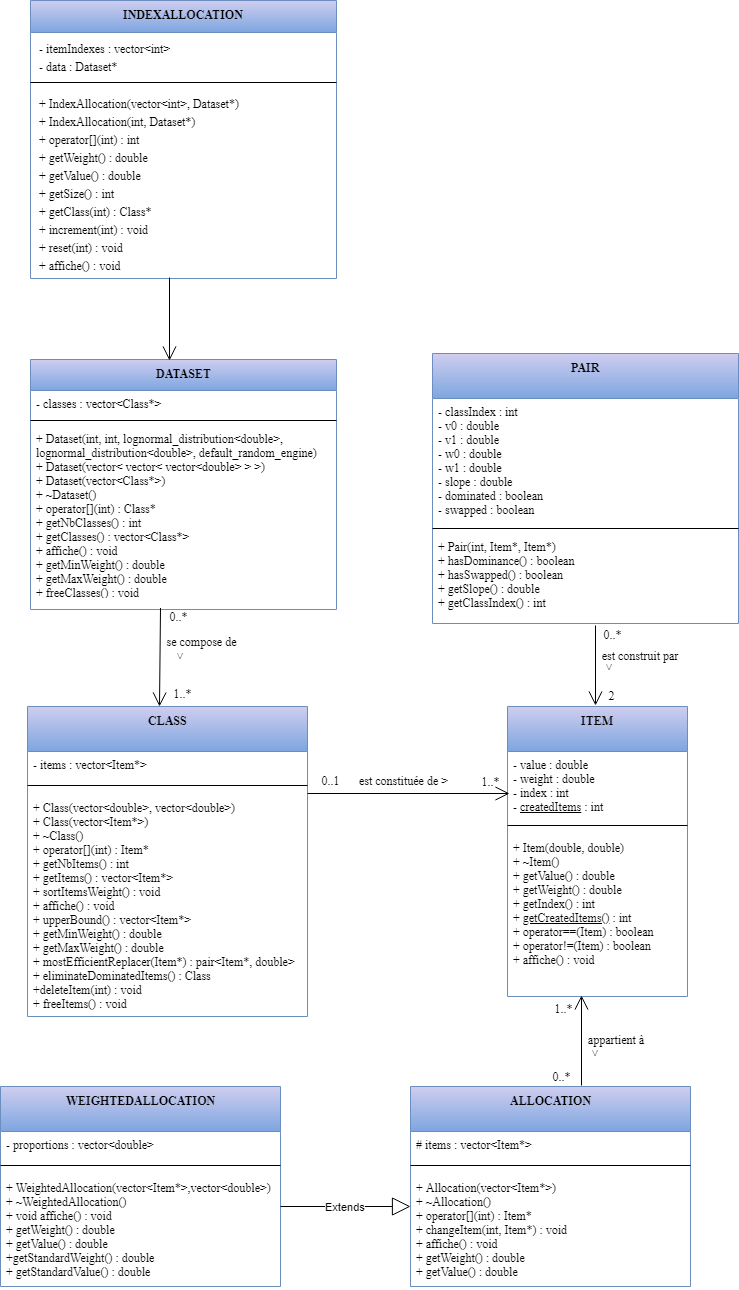
\includegraphics[width=12cm]{KnapsackClasses.png}
	\caption{Diagramme de classes}
	\label{fig:diagramme}
\end{figure}

\newpage
\section{Application économique}
% Je vais ici parler de l'application du MCKP à une politique d'incitation.

Le problème du sac à dos à choix multiple peut être appliqué à la politique économique.
Considérons l'analogie suivante :
\begin{itemize}
	\item Le sac à dos représente l'économie ou un secteur de l'économie.
	\item La capacité du sac à dos représente le budget du gouvernement.
	\item Les différentes classes représente les différents individus dans l'économie.
	\item Les objets de la classe $j$ représente les choix que peux faire l'individu $j$ (par ex., choix entre plusieurs modèles de voiture, choix entre plusieurs modes de transport).
	\item La valeur de l'objet $x$ représente le bénéfice social associé au choix de $x$.
	\item Le poids de l'objet $x$ représente l'opposé de l'utilité que retire l'individu s'il fait le choix $x$ (plus le poids est faible, plus l'utilité associée est grande).
\end{itemize}

Supposons que le gouvernement utilise son budget pour distribuer des incitations aux individus de la façon suivante : si l'individu choisit $x$ mais que le gouvernement souhaite qu'il choisisse $y$ (avec $w_x < w_y$), alors le gouvernement donne une incitation d'un montant $w_y - w_x$ à l'individu pour qu'il change son choix.\footnote{Le gouvernement ayant une information parfaite sur les utilités des individus, il peut proposer l'incitation qui suffit juste à convaincre l'individu de changer son choix.}
Si l'objectif du gouvernement est de maximiser la somme des bénéfices sociaux dans l'économie, alors la solution du MCKP concorde avec la solution du programme de maximisation du gouvernement.

L'allocation optimale retournée par les algorithmes du MCKP correspond au choix qui doit être fait par chaque individus.
Le montant des incitations distribué, pour chaque individu, est égal à la différence entre le poids de l'objet choisi à l'optimum et le poids de l'objet le plus léger (c'est le choix qui procure la plus grande utilité à l'individu).

\begin{thebibliography}{9}
\bibitem{Knapsack2004}
  Hans Kellerer, Ulrich Pferschy and David Pisinger,
  \textit{Knapsack problems},
  Springer,
  2004.
\end{thebibliography}

\end{document}
